% -----------------------------------------------------------------------------
%                                     HEADER                                    
% -----------------------------------------------------------------------------
\documentclass[a4paper, 10pt]{article}
\usepackage{jheppub}
\usepackage[T1]{fontenc}
\usepackage{colortbl,xcolor,float}
\definecolor{orange}{rgb}{1,0.5,0}
% -----------------------------------------------------------------------------
%                                   COVER PAGE                                  
% -----------------------------------------------------------------------------
\title{{
\includegraphics[scale=.4]{logo.eps}}\ The LaTeX report}

\author{Generated by s1412595 on 08 July 2019, 15:54:23}

\abstract{
  This report has been generated automatically
  by {\sc MadAnalysis} 5.\\$~$\\ 
  Please cite:\\ 
  \begin{quote}
    \textbf{E.~Conte, B.~Fuks and G.~Serret},\\ 
    \textit{MadAnalysis 5, A User-Friendly
    Framework for Collider Phenomenology},\\ 
    Comput. Phys. Commun. {\bf 184} (2013) 222-256,\\
    arXiv:1206.1599 [hep-ph].\\ 
  \end{quote}
  To contact us:\\ 
  \begin{quote}
    \textbf{http://madanalysis.irmp.ucl.ac.be}\\
    \textbf{ma5team@iphc.cnrs.fr}\\
  \end{quote}
}

% -----------------------------------------------------------------------------
%                                 BEGIN DOCUMENT                                
% -----------------------------------------------------------------------------
\begin{document}
\maketitle
\flushbottom

% -----------------------------------------------------------------------------
%                                 SECTION Setup                                 
% -----------------------------------------------------------------------------
\newpage
\section{ Setup}

\subsection{ Command history}

\texttt{ma5>import /\-home/\-s1412595/\-Desktop/\-SummerProject2019/\-MG5\_aMC\_v2\_6\_6/\-BP2\_080719/\-bin/\-internal/\-ufomodel\\
}
\texttt{ }\texttt{ }\texttt{ma5>import /\-home/\-s1412595/\-Desktop/\-SummerProject2019/\-MG5\_aMC\_v2\_6\_6/\-BP2\_080719/\-Events/\-run\_01/\-unweighted\_events.lhe.gz as unweighted\_events\\
}
\texttt{ }\texttt{ }\texttt{ma5>define vl = 12 14 16\\
}
\texttt{ }\texttt{ }\texttt{ma5>define vl~ = -16 -14 -12\\
}
\texttt{ }\texttt{ }\texttt{ma5>define invisible = ve ve~ vm vm~ vt vt~ vl vl~\\
}
\texttt{ }\texttt{ }\texttt{ma5>set main.graphic\_render = root\\
}
\texttt{ }\texttt{ }\texttt{ma5>plot THT   40 0 500 [logY]\\
}
\texttt{ }\texttt{ }\texttt{ma5>plot MET   40 0 500 [logY]\\
}
\texttt{ }\texttt{ }\texttt{ma5>plot SQRTS 40 0 500 [logY]\\
}
\texttt{ }\texttt{ }\texttt{ma5>plot  PT(~chi+[1]) 40 0  500 [logY interstate]\\
}
\texttt{ }\texttt{ }\texttt{ma5>plot ETA(~chi+[1]) 40 -10 10 [logY interstate]\\
}
\texttt{ }\texttt{ }\texttt{ma5>plot  PT(~chi-[1]) 40 0  500 [logY]\\
}
\texttt{ }\texttt{ }\texttt{ma5>plot ETA(~chi-[1]) 40 -10 10 [logY]\\
}
\texttt{ }\texttt{ }\texttt{ma5>plot M(~chi+[1] ~chi-[1]) 40 0  500 [logY allstate]\\
}
\texttt{ }\texttt{ }\texttt{ma5>plot DELTAR(~chi+[1],~chi-[1]) 40 0 10 [logY allstate]\\
}
\texttt{ }\texttt{ }\texttt{ma5>plot  PT(~chi-[1]) 40 0  500 [logY]\\
}
\texttt{ }\texttt{ }\texttt{ma5>plot ETA(~chi-[1]) 40 -10 10 [logY]\\
}
\texttt{ }\texttt{ }\texttt{ma5>plot  PT(~psi[1]) 40 0  500 [logY]\\
}
\texttt{ }\texttt{ }\texttt{ma5>plot ETA(~psi[1]) 40 -10 10 [logY]\\
}
\texttt{ }\texttt{ }\texttt{ma5>plot  PT(l+[1]) 40 0  500 [logY]\\
}
\texttt{ }\texttt{ }\texttt{ma5>plot ETA(l+[1]) 40 -10 10 [logY]\\
}
\texttt{ }\texttt{ }\texttt{ma5>plot  PT(nn[1]) 40 0  500 [logY]\\
}
\texttt{ }\texttt{ }\texttt{ma5>plot ETA(nn[1]) 40 -10 10 [logY]\\
}
\texttt{ }\texttt{ }\texttt{ma5>plot M(l+[1] nn[1]) 40 0  500 [logY ]\\
}
\texttt{ }\texttt{ }\texttt{ma5>plot M(~chi-[1] l+[1]) 40 0  500 [logY ]\\
}
\texttt{ }\texttt{ }\texttt{ma5>plot M(~chi-[1] l+[1] nn[1]) 40 0  500 [logY ]\\
}
\texttt{ }\texttt{ }\texttt{ma5>plot M(~chi-[1] nn[1]) 40 0  500 [logY ]\\
}
\texttt{ }\texttt{ }\texttt{ma5>plot M(~chi-[1] ~psi[1]) 40 0  500 [logY ]\\
}
\texttt{ }\texttt{ }\texttt{ma5>plot M(~chi-[1] ~psi[1] l+[1]) 40 0  500 [logY ]\\
}
\texttt{ }\texttt{ }\texttt{ma5>plot M(~chi-[1] ~psi[1] l+[1] nn[1]) 40 0  500 [logY ]\\
}
\texttt{ }\texttt{ }\texttt{ma5>plot M(~chi-[1] ~psi[1] nn[1]) 40 0  500 [logY ]\\
}
\texttt{ }\texttt{ }\texttt{ma5>plot M(~psi[1] l+[1]) 40 0  500 [logY ]\\
}
\texttt{ }\texttt{ }\texttt{ma5>plot M(~psi[1] l+[1] nn[1]) 40 0  500 [logY ]\\
}
\texttt{ }\texttt{ }\texttt{ma5>plot M(~psi[1] nn[1]) 40 0  500 [logY ]\\
}
\texttt{ }\texttt{ }\texttt{ma5>plot DELTAR(l+[1],nn[1]) 40 0 10 [logY ]\\
}
\texttt{ }\texttt{ }\texttt{ma5>plot DELTAR(~chi-[1],l+[1]) 40 0 10 [logY ]\\
}
\texttt{ }\texttt{ }\texttt{ma5>plot DELTAR(~chi-[1],nn[1]) 40 0 10 [logY ]\\
}
\texttt{ }\texttt{ }\texttt{ma5>plot DELTAR(~chi-[1],~psi[1]) 40 0 10 [logY ]\\
}
\texttt{ }\texttt{ }\texttt{ma5>plot DELTAR(~psi[1],l+[1]) 40 0 10 [logY ]\\
}
\texttt{ }\texttt{ }\texttt{ma5>plot DELTAR(~psi[1],nn[1]) 40 0 10 [logY ]\\
}
\texttt{ }\texttt{ }\texttt{ma5>plot  PT(~chi-[1]) 40 0  500 [logY interstate]\\
}
\texttt{ }\texttt{ }\texttt{ma5>plot ETA(~chi-[1]) 40 -10 10 [logY interstate]\\
}
\texttt{ }\texttt{ }\texttt{ma5>plot  PT(~chi+[1]) 40 0  500 [logY]\\
}
\texttt{ }\texttt{ }\texttt{ma5>plot ETA(~chi+[1]) 40 -10 10 [logY]\\
}
\texttt{ }\texttt{ }\texttt{ma5>plot M(~chi-[1] ~chi+[1]) 40 0  500 [logY allstate]\\
}
\texttt{ }\texttt{ }\texttt{ma5>plot DELTAR(~chi-[1],~chi+[1]) 40 0 10 [logY allstate]\\
}
\texttt{ }\texttt{ }\texttt{ma5>plot  PT(~psi~[1]) 40 0  500 [logY]\\
}
\texttt{ }\texttt{ }\texttt{ma5>plot ETA(~psi~[1]) 40 -10 10 [logY]\\
}
\texttt{ }\texttt{ }\texttt{ma5>plot  PT(l-[1]) 40 0  500 [logY]\\
}
\texttt{ }\texttt{ }\texttt{ma5>plot ETA(l-[1]) 40 -10 10 [logY]\\
}
\texttt{ }\texttt{ }\texttt{ma5>plot  PT(~chi+[1]) 40 0  500 [logY]\\
}
\texttt{ }\texttt{ }\texttt{ma5>plot ETA(~chi+[1]) 40 -10 10 [logY]\\
}
\texttt{ }\texttt{ }\texttt{ma5>plot  PT(nn~[1]) 40 0  500 [logY]\\
}
\texttt{ }\texttt{ }\texttt{ma5>plot ETA(nn~[1]) 40 -10 10 [logY]\\
}
\texttt{ }\texttt{ }\texttt{ma5>plot M(l-[1] nn~[1]) 40 0  500 [logY ]\\
}
\texttt{ }\texttt{ }\texttt{ma5>plot M(l-[1] ~chi+[1]) 40 0  500 [logY ]\\
}
\texttt{ }\texttt{ }\texttt{ma5>plot M(l-[1] ~chi+[1] nn~[1]) 40 0  500 [logY ]\\
}
\texttt{ }\texttt{ }\texttt{ma5>plot M(~chi+[1] nn~[1]) 40 0  500 [logY ]\\
}
\texttt{ }\texttt{ }\texttt{ma5>plot M(~psi~[1] l-[1]) 40 0  500 [logY ]\\
}
\texttt{ }\texttt{ }\texttt{ma5>plot M(~psi~[1] l-[1] nn~[1]) 40 0  500 [logY ]\\
}
\texttt{ }\texttt{ }\texttt{ma5>plot M(~psi~[1] l-[1] ~chi+[1]) 40 0  500 [logY ]\\
}
\texttt{ }\texttt{ }\texttt{ma5>plot M(~psi~[1] l-[1] ~chi+[1] nn~[1]) 40 0  500 [logY ]\\
}
\texttt{ }\texttt{ }\texttt{ma5>plot M(~psi~[1] nn~[1]) 40 0  500 [logY ]\\
}
\texttt{ }\texttt{ }\texttt{ma5>plot M(~psi~[1] ~chi+[1]) 40 0  500 [logY ]\\
}
\texttt{ }\texttt{ }\texttt{ma5>plot M(~psi~[1] ~chi+[1] nn~[1]) 40 0  500 [logY ]\\
}
\texttt{ }\texttt{ }\texttt{ma5>plot DELTAR(l-[1],nn~[1]) 40 0 10 [logY ]\\
}
\texttt{ }\texttt{ }\texttt{ma5>plot DELTAR(l-[1],~chi+[1]) 40 0 10 [logY ]\\
}
\texttt{ }\texttt{ }\texttt{ma5>plot DELTAR(~chi+[1],nn~[1]) 40 0 10 [logY ]\\
}
\texttt{ }\texttt{ }\texttt{ma5>plot DELTAR(~psi~[1],l-[1]) 40 0 10 [logY ]\\
}
\texttt{ }\texttt{ }\texttt{ma5>plot DELTAR(~psi~[1],nn~[1]) 40 0 10 [logY ]\\
}
\texttt{ }\texttt{ }\texttt{ma5>plot DELTAR(~psi~[1],~chi+[1]) 40 0 10 [logY ]\\
}
\texttt{ }\texttt{ }\texttt{ma5>submit /\-home/\-s1412595/\-Desktop/\-SummerProject2019/\-MG5\_aMC\_v2\_6\_6/\-BP2\_080719/\-MA5\_PARTON\_ANALYSIS\_analysis1\\
}
\texttt{ }\texttt{ }\subsection{ Configuration}

\begin{itemize}
  \item MadAnalysis version 1.8.5 (2019/\-04/\-04).
   \item Histograms given for an integrated luminosity of \textcolor{blue}{10}\textcolor{blue}{ fb}$^{\textcolor{blue}{-1}}$\textcolor{blue}{.}
\textcolor{blue}{}
\end{itemize}
% -----------------------------------------------------------------------------
%                                SECTION Datasets                               
% -----------------------------------------------------------------------------
\newpage
\section{ Datasets}

\subsection{ unweighted\_events}

\begin{itemize}
  \item Sample consisting of: \textcolor{blue}{signal}  events.
   \item Generated events: \textcolor{blue}{1000 }  events.
   \item Normalization to the luminosity: \textcolor{blue}{0}\textcolor{blue}{ +/\-- }\textcolor{blue}{1 }  events.
   \item Ratio (event weight): \textcolor{blue}{0.0 } .  
 
\end{itemize}
\begin{table}[H]
  \begin{center}
    \begin{tabular}{|m{55.0mm}|m{25.0mm}|m{30.0mm}|m{30.0mm}|}
      \hline
      {\cellcolor{yellow}         Path to the event file}& {\cellcolor{yellow}         Nr. of events}& {\cellcolor{yellow}         Cross section (pb)}& {\cellcolor{yellow}         Negative wgts (\%)}\\
      \hline
      {\cellcolor{white}          Events/\-run\_01/\-unweighted\_events.lhe.gz}& {\cellcolor{white}          1000}& {\cellcolor{white}          4.93e-49 @ 0.73\%}& {\cellcolor{white}          0.0}\\
\hline
    \end{tabular}
  \end{center}
\end{table}

% -----------------------------------------------------------------------------
%                            SECTION Histos and cuts                            
% -----------------------------------------------------------------------------
\newpage
\section{ Histos and cuts}

\subsection{ Histogram 1}

\textbf{* Plot: THT}\\
   \begin{table}[H]
  \begin{center}
    \begin{tabular}{|m{23.0mm}|m{23.0mm}|m{18.0mm}|m{19.0mm}|m{19.0mm}|m{19.0mm}|m{19.0mm}|}
      \hline
      {\cellcolor{yellow}         Dataset}& {\cellcolor{yellow}         Integral}& {\cellcolor{yellow}         Entries per event}& {\cellcolor{yellow}         Mean}& {\cellcolor{yellow}         RMS}& {\cellcolor{yellow}         \% underflow}& {\cellcolor{yellow}         \% overflow}\\
      \hline
      {\cellcolor{white}         unweighted\_events}& {\cellcolor{white}         0.0 +/\-- 0.0}& {\cellcolor{white}         1.0}& {\cellcolor{white}         0.0}& {\cellcolor{white}         0.0}& {\cellcolor{green}         0.0}& {\cellcolor{green}         0.0}\\
\hline
    \end{tabular}
  \end{center}
\end{table}

\begin{figure}[H]
  \begin{center}
    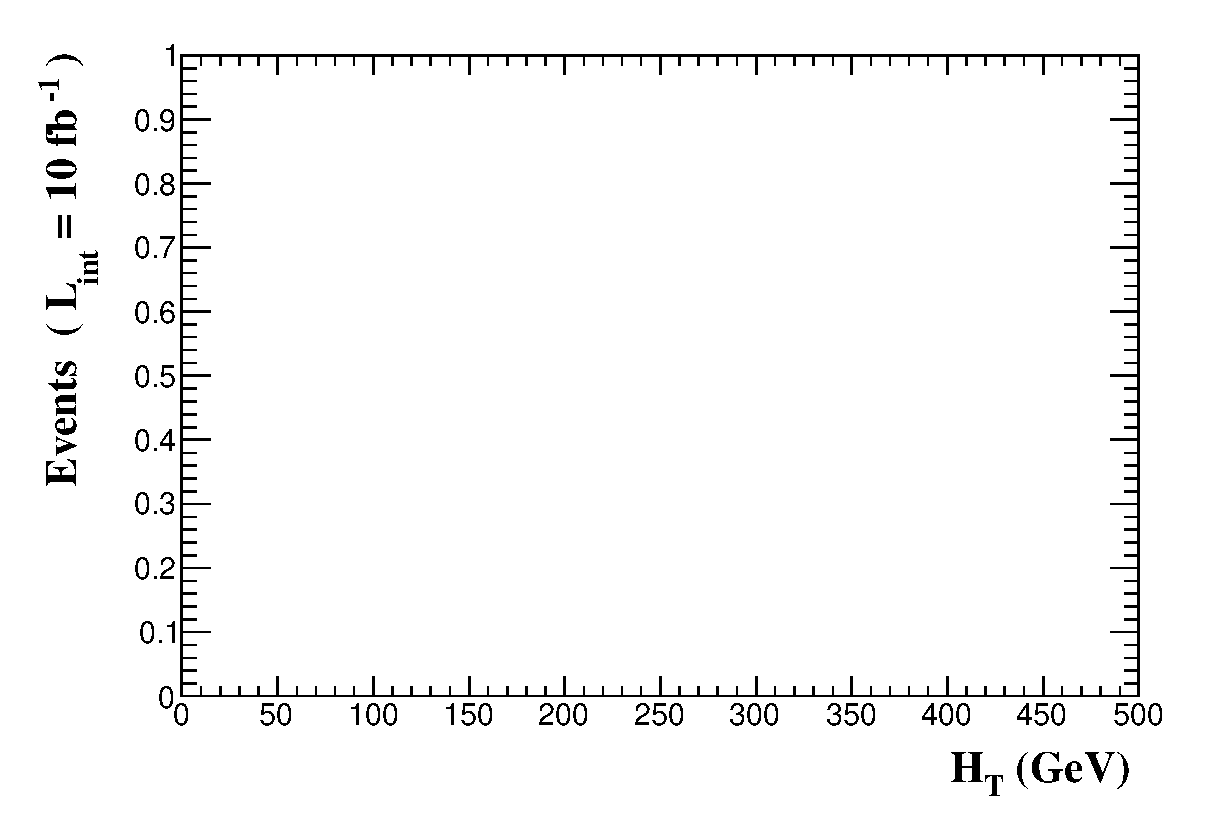
\includegraphics[scale=0.45]{selection_0.eps}\\
\caption{   }
  \end{center}
\end{figure}
      \newpage
\subsection{ Histogram 2}

\textbf{* Plot: MET}\\
   \begin{table}[H]
  \begin{center}
    \begin{tabular}{|m{23.0mm}|m{23.0mm}|m{18.0mm}|m{19.0mm}|m{19.0mm}|m{19.0mm}|m{19.0mm}|}
      \hline
      {\cellcolor{yellow}         Dataset}& {\cellcolor{yellow}         Integral}& {\cellcolor{yellow}         Entries per event}& {\cellcolor{yellow}         Mean}& {\cellcolor{yellow}         RMS}& {\cellcolor{yellow}         \% underflow}& {\cellcolor{yellow}         \% overflow}\\
      \hline
      {\cellcolor{white}         unweighted\_events}& {\cellcolor{white}         0.0 +/\-- 0.0}& {\cellcolor{white}         1.0}& {\cellcolor{white}         0.0}& {\cellcolor{white}         0.0}& {\cellcolor{green}         0.0}& {\cellcolor{green}         0.0}\\
\hline
    \end{tabular}
  \end{center}
\end{table}

\begin{figure}[H]
  \begin{center}
    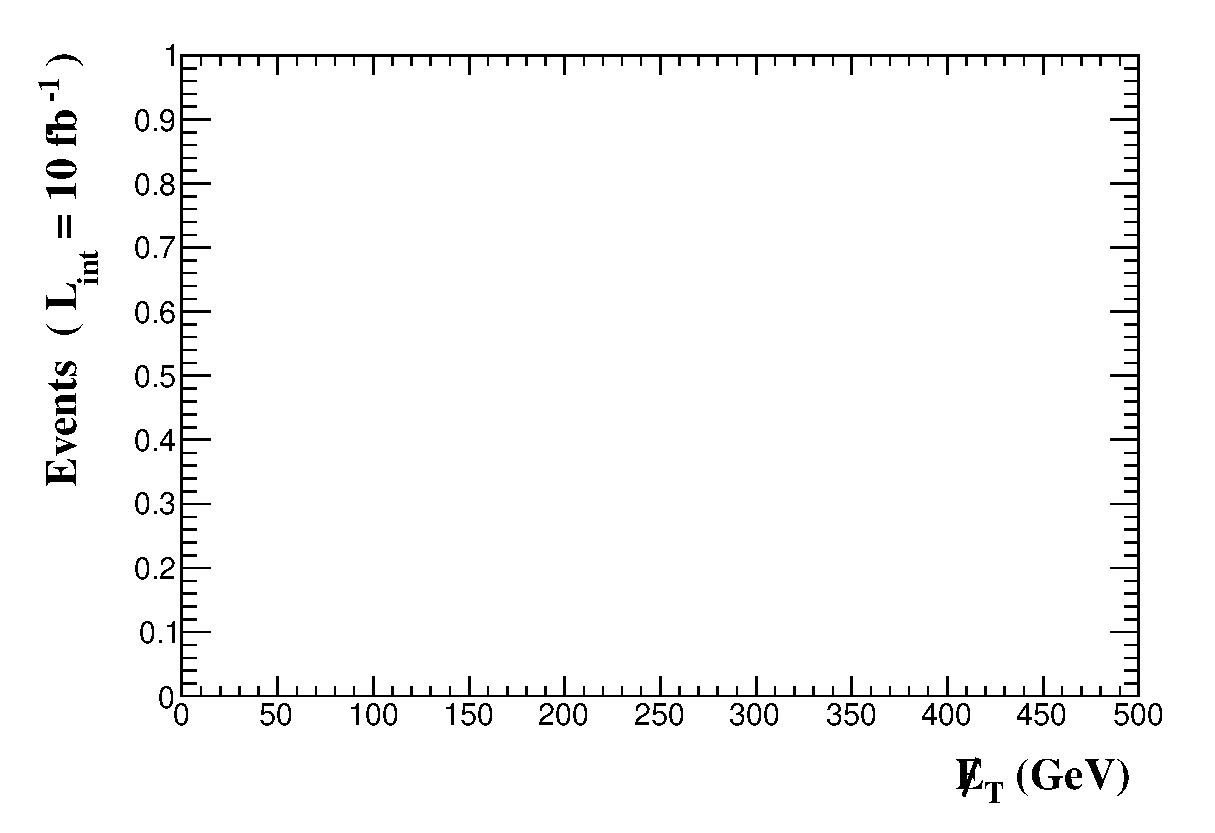
\includegraphics[scale=0.45]{selection_1.eps}\\
\caption{   }
  \end{center}
\end{figure}
      \newpage
\subsection{ Histogram 3}

\textbf{* Plot: SQRTS}\\
   \begin{table}[H]
  \begin{center}
    \begin{tabular}{|m{23.0mm}|m{23.0mm}|m{18.0mm}|m{19.0mm}|m{19.0mm}|m{19.0mm}|m{19.0mm}|}
      \hline
      {\cellcolor{yellow}         Dataset}& {\cellcolor{yellow}         Integral}& {\cellcolor{yellow}         Entries per event}& {\cellcolor{yellow}         Mean}& {\cellcolor{yellow}         RMS}& {\cellcolor{yellow}         \% underflow}& {\cellcolor{yellow}         \% overflow}\\
      \hline
      {\cellcolor{white}         unweighted\_events}& {\cellcolor{white}         0.0 +/\-- 0.0}& {\cellcolor{white}         1.0}& {\cellcolor{white}         0.0}& {\cellcolor{white}         0.0}& {\cellcolor{green}         0.0}& {\cellcolor{green}         0.0}\\
\hline
    \end{tabular}
  \end{center}
\end{table}

\begin{figure}[H]
  \begin{center}
    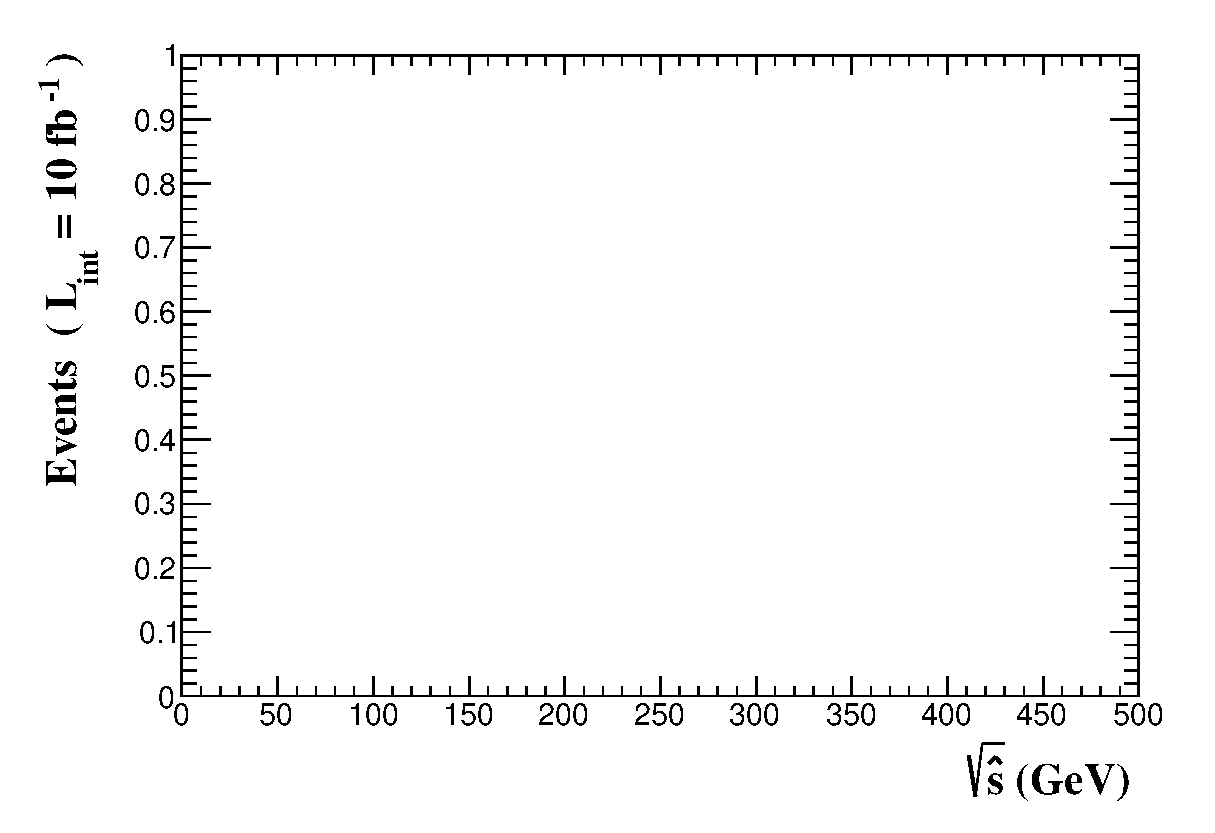
\includegraphics[scale=0.45]{selection_2.eps}\\
\caption{   }
  \end{center}
\end{figure}
      \newpage
\subsection{ Histogram 4}

\textbf{* Plot: PT ( l+[1] ) }\\
   \begin{table}[H]
  \begin{center}
    \begin{tabular}{|m{23.0mm}|m{23.0mm}|m{18.0mm}|m{19.0mm}|m{19.0mm}|m{19.0mm}|m{19.0mm}|}
      \hline
      {\cellcolor{yellow}         Dataset}& {\cellcolor{yellow}         Integral}& {\cellcolor{yellow}         Entries per event}& {\cellcolor{yellow}         Mean}& {\cellcolor{yellow}         RMS}& {\cellcolor{yellow}         \% underflow}& {\cellcolor{yellow}         \% overflow}\\
      \hline
      {\cellcolor{white}         unweighted\_events}& {\cellcolor{white}         0.0 +/\-- 0.0}& {\cellcolor{white}         1.0}& {\cellcolor{white}         0.0}& {\cellcolor{white}         0.0}& {\cellcolor{green}         0.0}& {\cellcolor{green}         0.0}\\
\hline
    \end{tabular}
  \end{center}
\end{table}

\begin{figure}[H]
  \begin{center}
    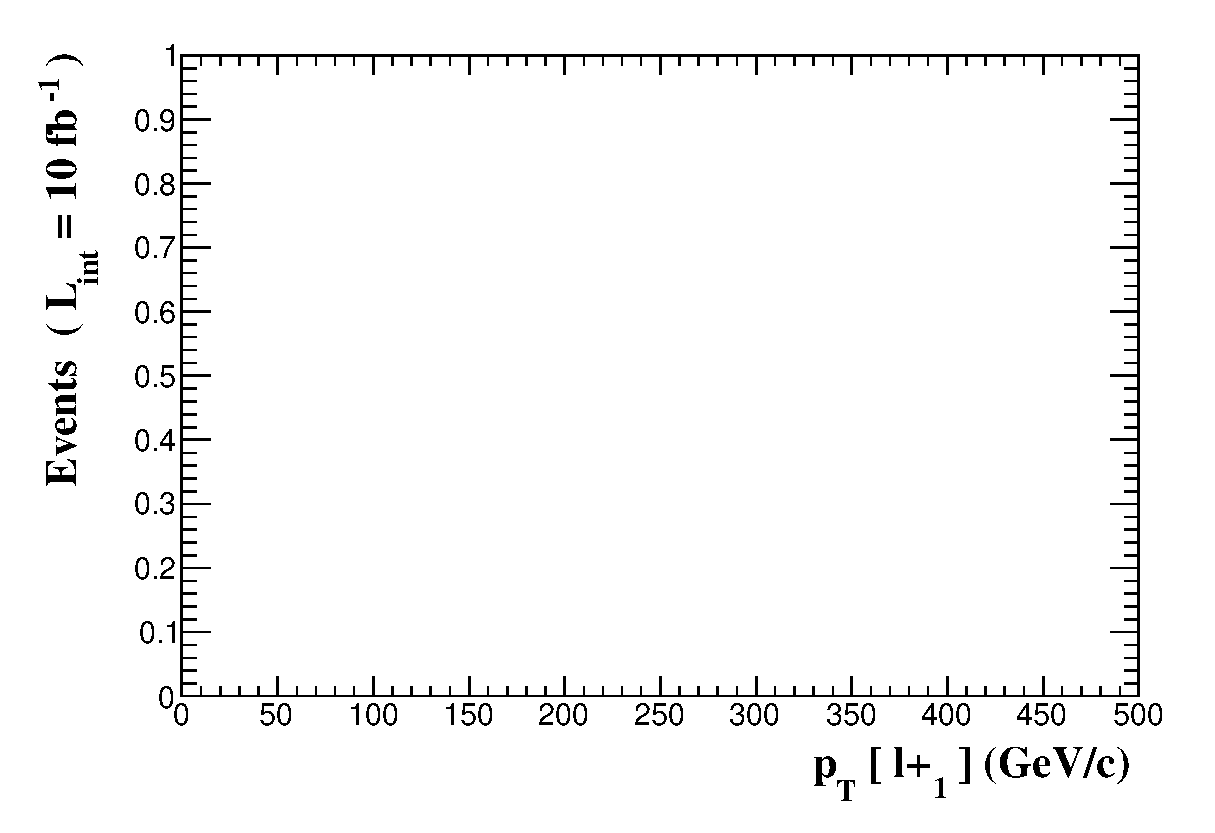
\includegraphics[scale=0.45]{selection_3.eps}\\
\caption{   }
  \end{center}
\end{figure}
      \newpage
\subsection{ Histogram 5}

\textbf{* Plot: ETA ( l+[1] ) }\\
   \begin{table}[H]
  \begin{center}
    \begin{tabular}{|m{23.0mm}|m{23.0mm}|m{18.0mm}|m{19.0mm}|m{19.0mm}|m{19.0mm}|m{19.0mm}|}
      \hline
      {\cellcolor{yellow}         Dataset}& {\cellcolor{yellow}         Integral}& {\cellcolor{yellow}         Entries per event}& {\cellcolor{yellow}         Mean}& {\cellcolor{yellow}         RMS}& {\cellcolor{yellow}         \% underflow}& {\cellcolor{yellow}         \% overflow}\\
      \hline
      {\cellcolor{white}         unweighted\_events}& {\cellcolor{white}         0.0 +/\-- 0.0}& {\cellcolor{white}         1.0}& {\cellcolor{white}         0.0}& {\cellcolor{white}         0.0}& {\cellcolor{green}         0.0}& {\cellcolor{green}         0.0}\\
\hline
    \end{tabular}
  \end{center}
\end{table}

\begin{figure}[H]
  \begin{center}
    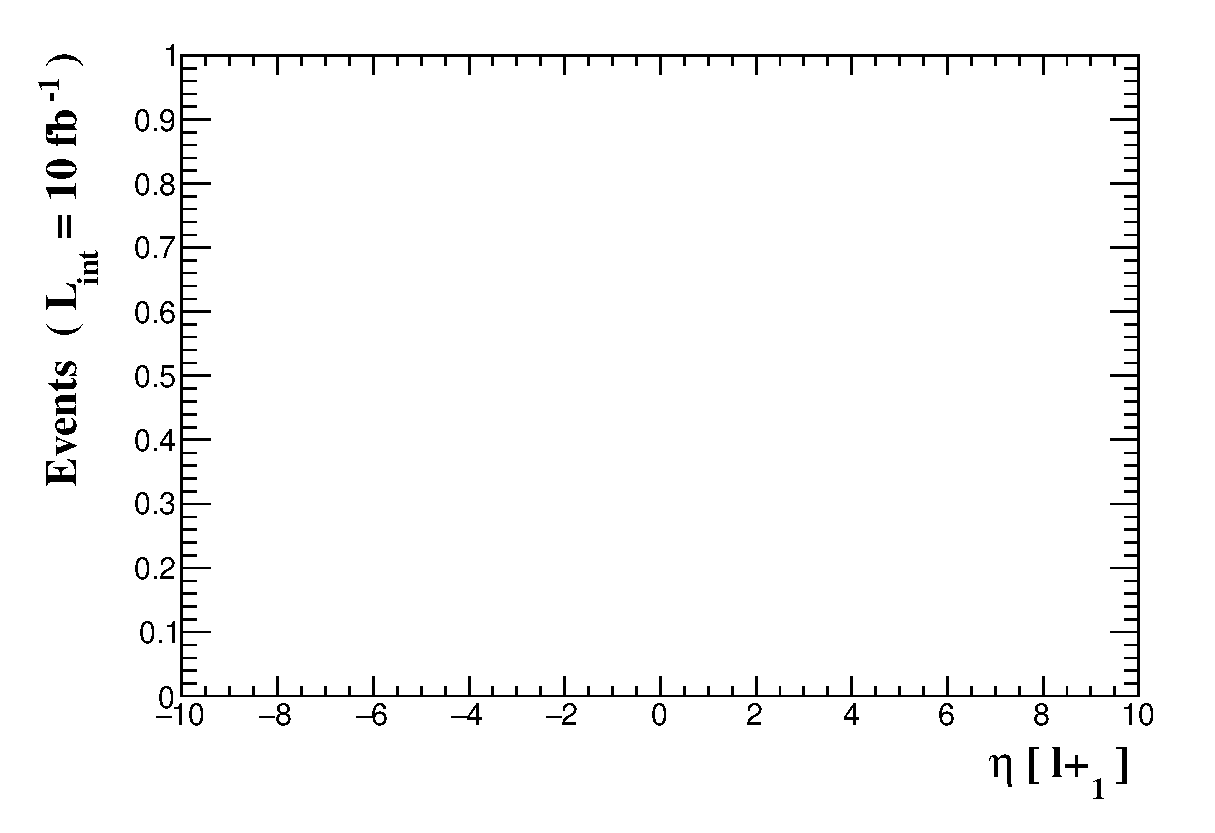
\includegraphics[scale=0.45]{selection_4.eps}\\
\caption{   }
  \end{center}
\end{figure}
      \newpage
\subsection{ Histogram 6}

\textbf{* Plot: PT ( l-[1] ) }\\
   \begin{table}[H]
  \begin{center}
    \begin{tabular}{|m{23.0mm}|m{23.0mm}|m{18.0mm}|m{19.0mm}|m{19.0mm}|m{19.0mm}|m{19.0mm}|}
      \hline
      {\cellcolor{yellow}         Dataset}& {\cellcolor{yellow}         Integral}& {\cellcolor{yellow}         Entries per event}& {\cellcolor{yellow}         Mean}& {\cellcolor{yellow}         RMS}& {\cellcolor{yellow}         \% underflow}& {\cellcolor{yellow}         \% overflow}\\
      \hline
      {\cellcolor{white}         unweighted\_events}& {\cellcolor{white}         0.0 +/\-- 0.0}& {\cellcolor{white}         1.0}& {\cellcolor{white}         0.0}& {\cellcolor{white}         0.0}& {\cellcolor{green}         0.0}& {\cellcolor{green}         0.0}\\
\hline
    \end{tabular}
  \end{center}
\end{table}

\begin{figure}[H]
  \begin{center}
    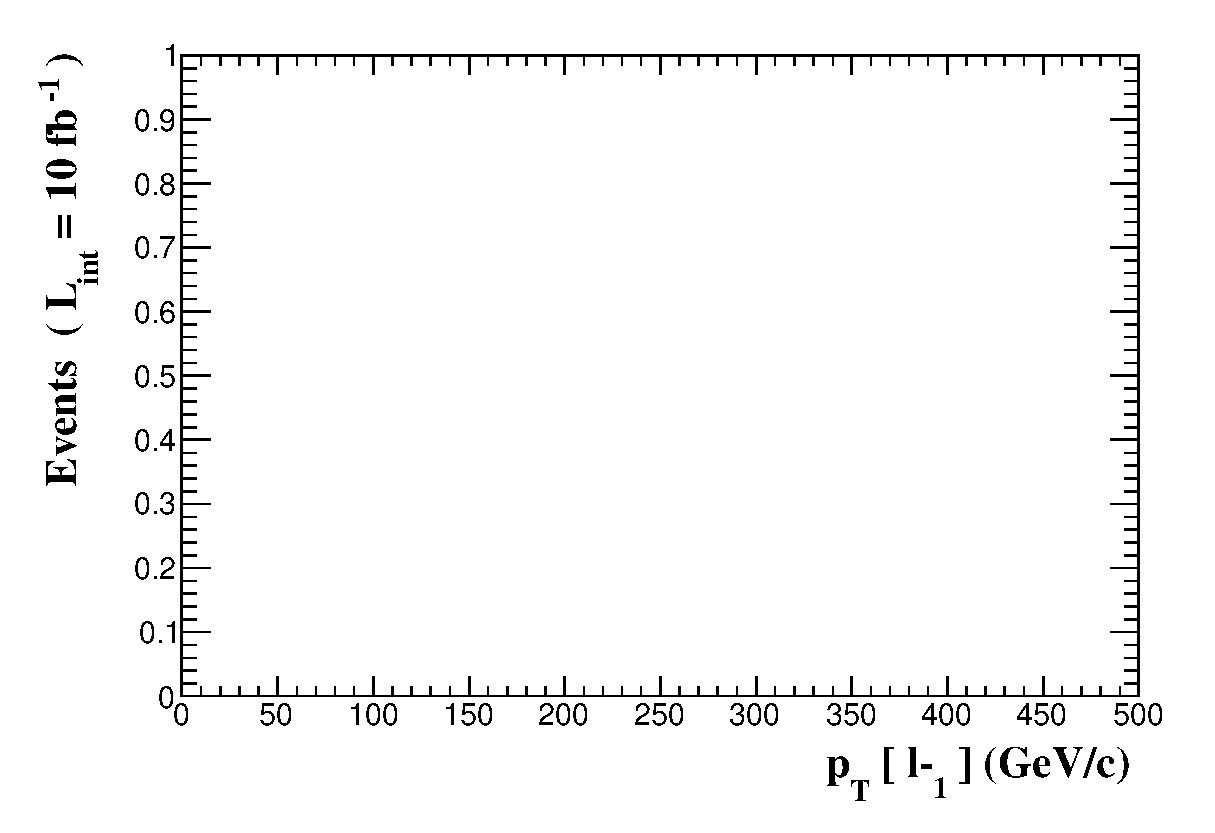
\includegraphics[scale=0.45]{selection_5.eps}\\
\caption{   }
  \end{center}
\end{figure}
      \newpage
\subsection{ Histogram 7}

\textbf{* Plot: ETA ( l-[1] ) }\\
   \begin{table}[H]
  \begin{center}
    \begin{tabular}{|m{23.0mm}|m{23.0mm}|m{18.0mm}|m{19.0mm}|m{19.0mm}|m{19.0mm}|m{19.0mm}|}
      \hline
      {\cellcolor{yellow}         Dataset}& {\cellcolor{yellow}         Integral}& {\cellcolor{yellow}         Entries per event}& {\cellcolor{yellow}         Mean}& {\cellcolor{yellow}         RMS}& {\cellcolor{yellow}         \% underflow}& {\cellcolor{yellow}         \% overflow}\\
      \hline
      {\cellcolor{white}         unweighted\_events}& {\cellcolor{white}         0.0 +/\-- 0.0}& {\cellcolor{white}         1.0}& {\cellcolor{white}         0.0}& {\cellcolor{white}         0.0}& {\cellcolor{green}         0.0}& {\cellcolor{green}         0.0}\\
\hline
    \end{tabular}
  \end{center}
\end{table}

\begin{figure}[H]
  \begin{center}
    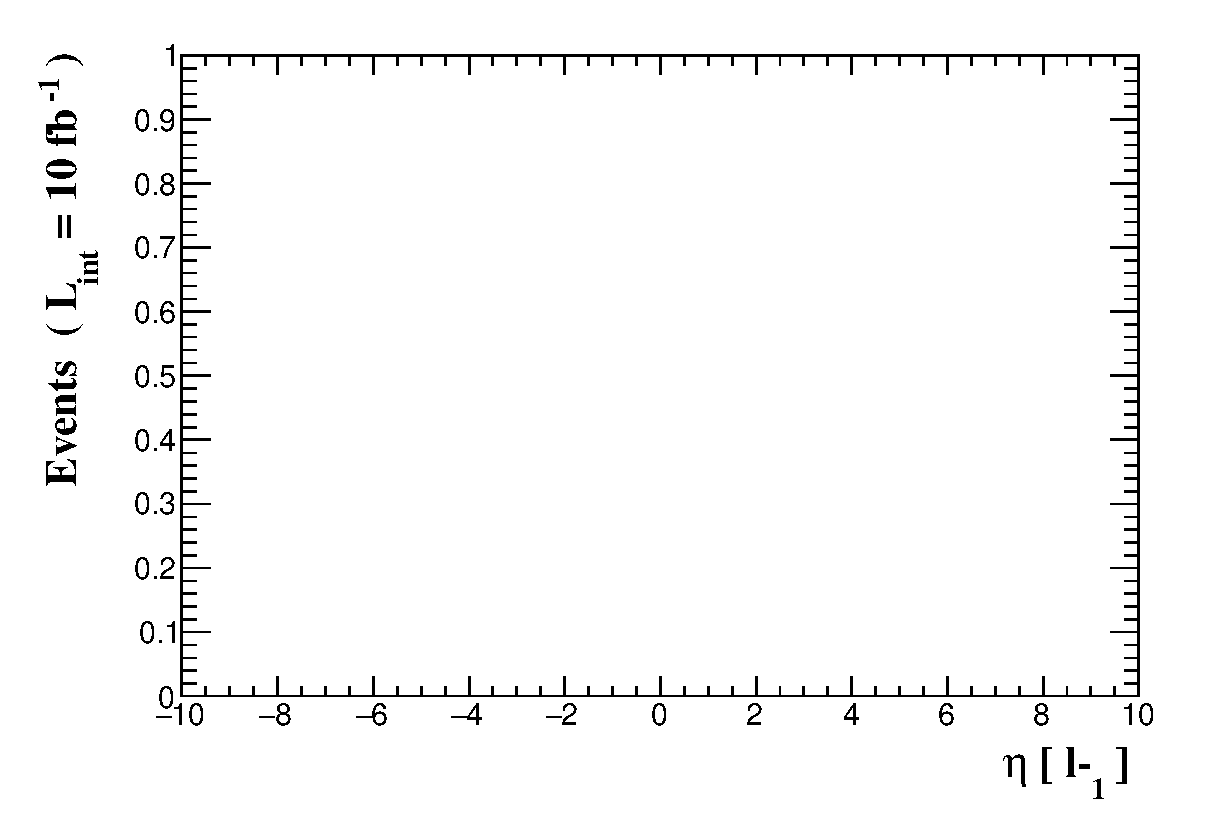
\includegraphics[scale=0.45]{selection_6.eps}\\
\caption{   }
  \end{center}
\end{figure}
      \end{document}
